% Manuskrip EPW 17: sumber tunggal, bibliografi inline, gambar placeholder.
% Abstrak dipertahankan verbatim dari naskah yang telah lolos seleksi.
% Data: 60 sesi utama / 30 pasangan, sumber 62be1a5a, audit 29 September 2026.
\documentclass[10pt,a4paper]{article}
\usepackage[top=2.54cm,left=2.54cm,right=2.54cm,bottom=3cm]{geometry}
\usepackage{iftex}
\usepackage{mathptmx}
\ifPDFTeX
  \usepackage[T1]{fontenc}
  \usepackage[utf8]{inputenc}
  \typeout{EPW-FONT: Times-compatible (mathptmx).}
\else
  \usepackage{fontspec}
  % Font paket dipilih melalui nama file; compiler bawaan membatasi font sistem.
  \setmainfont{texgyretermes-regular.otf}[BoldFont=texgyretermes-bold.otf,ItalicFont=texgyretermes-italic.otf,BoldItalicFont=texgyretermes-bolditalic.otf]
  \typeout{EPW-FONT: TeX Gyre Termes (Times-compatible).}
\fi
\usepackage{amsmath}
\usepackage{array,booktabs,tabularx,longtable}
\usepackage{graphicx}
\usepackage{subcaption}
\graphicspath{{figures/}}
\usepackage{tikz}
\usetikzlibrary{arrows.meta}
\usepackage{setspace,titlesec,caption,cite,ragged2e}
\usepackage[section]{placeins}
\usepackage[hidelinks]{hyperref}
\usepackage{url}
\urlstyle{same}
\hypersetup{pdftitle={SAFE-MINING EVAC: Simulasi Navigasi Evakuasi Adaptif},pdfauthor={Maulana Chandra Irawan; Khoirul Yardan Mauluddin Zhorif; Bagus Insan Pradana},pdfsubject={Naskah EPW 17 berdasarkan eksperimen Unity/Python/MQTT}}
\setlength{\parindent}{5mm}
\setlength{\parskip}{0pt}
\setlength{\emergencystretch}{1.5em}
\titleformat{\section}{\fontsize{11}{13}\selectfont\bfseries}{}{0pt}{}
\titleformat{\subsection}{\fontsize{10}{12}\selectfont\bfseries}{}{0pt}{}
\titlespacing*{\section}{0pt}{10pt}{5pt}
\titlespacing*{\subsection}{0pt}{7pt}{3pt}
\captionsetup{font=normalsize,labelfont=normalfont,labelsep=period,justification=centering,skip=5pt}
\renewcommand{\figurename}{Gambar}
\renewcommand{\tablename}{Tabel}
\renewcommand{\refname}{Referensi}
\setlength{\textfloatsep}{9pt}
\setlength{\intextsep}{8pt}
\setlength{\floatsep}{8pt}
\renewcommand{\arraystretch}{1.12}
\newcolumntype{Y}{>{\RaggedRight\arraybackslash}X}
\newcommand{\placeholder}[3]{%
 \begin{figure}[!htbp]\centering
 \fbox{\parbox[c][30mm][c]{0.94\linewidth}{\centering\textbf{PLACEHOLDER GAMBAR}\\[3pt]#1}}
 \caption{#2}\label{#3}\end{figure}}
\begin{document}
\begin{center}
{\fontsize{16}{18}\selectfont\bfseries \emph{Towards} SAFE-MINING EVAC: Perancangan Simulasi Navigasi Evakuasi Adaptif Berbasis Unity dan \emph{Edge Intelligence} pada Area Tambang Bawah Tanah\par}
\vspace{8pt}
{\fontsize{11}{13}\selectfont
Maulana Chandra Irawan\textsuperscript{1}, Khoirul Yardan Mauluddin Zhorif\textsuperscript{1},\\
Bagus Insan Pradana\textsuperscript{1}\par
\vspace{4pt}
\textsuperscript{1}Teknik Informatika, Departemen Teknik Informatika dan Komputer,\\
Politeknik Elektronika Negeri Surabaya\par
Jalan Raya ITS, Keputih, Kecamatan Sukolilo, Kota Surabaya (60111),\\
Jawa Timur, Indonesia\par
Email: \href{mailto:irawan@it.student.pens.ac.id}{irawan@it.student.pens.ac.id}\par}
\end{center}
\vspace{4pt}
\begin{spacing}{1.5}
\noindent\textbf{Abstrak.} % BEGIN ACCEPTED ABSTRACT
Pertambangan bawah tanah merupakan lingkungan kerja dengan risiko keselamatan yang tinggi, terutama ketika terjadi keadaan darurat yang menyebabkan perubahan zona bahaya dan menyulitkan pekerja dalam menentukan jalur evakuasi yang aman. Sistem evakuasi statis memiliki keterbatasan karena jalur yang telah ditentukan sebelumnya dapat menjadi tidak sesuai ketika kondisi lingkungan berubah selama proses evakuasi. Penelitian ini bertujuan merancang dan mengevaluasi simulasi SAFE-MINING EVAC sebagai sistem navigasi evakuasi adaptif yang mampu menyesuaikan jalur berdasarkan perubahan kondisi bahaya dan posisi pekerja pada area tambang bawah tanah. Metode penelitian dilakukan melalui perancangan lingkungan tambang bawah tanah secara virtual menggunakan Unity, pemodelan posisi pekerja dan zona bahaya secara dinamis, serta implementasi algoritma dynamic path planning pada edge intelligence untuk menghasilkan jalur evakuasi yang adaptif. Skenario simulasi dirancang dengan memberikan perubahan posisi dan tingkat bahaya pada titik tertentu sehingga sistem harus melakukan perhitungan ulang jalur menuju zona aman. Komunikasi data antara komponen simulasi dirancang menggunakan protokol MQTT atau WebSocket untuk merepresentasikan pertukaran informasi antara lingkungan tambang, modul pemrosesan, dan sistem navigasi. Validasi dilakukan dengan membandingkan kinerja jalur evakuasi dinamis terhadap jalur evakuasi statis sebagai baseline berdasarkan waktu tempuh, tingkat keamanan jalur, jumlah perubahan rute, dan waktu respons sistem terhadap perubahan kondisi bahaya. Hasil yang diharapkan berupa simulasi yang mampu menunjukkan kemampuan sistem dalam memperbarui jalur evakuasi secara adaptif ketika terjadi perubahan kondisi lingkungan serta memberikan jalur yang lebih sesuai terhadap situasi terkini dibandingkan pendekatan statis. Penelitian ini diharapkan dapat menjadi dasar pengembangan SAFE-MINING EVAC pada tahap berikutnya melalui integrasi perangkat keras, sistem lokalisasi pekerja, dan sensor lingkungan pada lingkungan tambang nyata. Dengan demikian, kontribusi penelitian ini terletak pada perancangan dan validasi awal mekanisme navigasi evakuasi adaptif melalui simulasi yang dapat digunakan untuk menguji kelayakan pendekatan sebelum diterapkan pada sistem fisik.
% END ACCEPTED ABSTRACT
\end{spacing}
\vspace{4pt}
\noindent\textbf{Kata Kunci:} Tambang Bawah Tanah; Navigasi Evakuasi; \emph{Dynamic Path Planning}; Unity; \emph{Edge Intelligence}

\section*{Pendahuluan}
Pertambangan bawah tanah merupakan lingkungan kerja yang kompleks dan memiliki tantangan keselamatan tinggi, terutama ketika terjadi keadaan darurat yang dapat mengubah kondisi jalur, mempersulit orientasi pekerja, dan membatasi akses menuju zona aman. Dalam kondisi tersebut, keberadaan informasi mengenai kondisi lingkungan dan posisi pekerja menjadi penting untuk mendukung pengambilan keputusan evakuasi. Penelitian mengenai \emph{Internet of Things-based command center} menunjukkan bahwa data kondisi lingkungan, posisi pekerja, dan peta tambang dapat diintegrasikan untuk mendukung respons keadaan darurat serta membantu menentukan lokasi evakuasi yang sesuai \cite{jha}. Namun, informasi tersebut perlu diproses secara cepat dan adaptif karena kondisi lingkungan tambang dapat berubah selama proses evakuasi berlangsung.

Pendekatan evakuasi berbasis pemodelan telah dikembangkan untuk mengatasi perubahan kondisi tersebut. Meij \emph{et al.} mengembangkan model evakuasi cerdas pada tambang bawah tanah dengan mempertimbangkan jalur yang terblokir dan karakteristik pekerja dalam menentukan rute evakuasi \cite{meij}. Sementara itu, Bi \emph{et al.} mengembangkan perencanaan rute evakuasi secara waktu nyata dengan mempertimbangkan perubahan kondisi bahaya seperti asap, karbon monoksida, dan temperatur sehingga jalur dapat disesuaikan terhadap kondisi keselamatan yang sedang berlangsung \cite{bi}. Penelitian tersebut menunjukkan bahwa penentuan rute evakuasi tidak cukup hanya menggunakan jalur terpendek, tetapi perlu mempertimbangkan perubahan kondisi lingkungan secara dinamis.

Selain kondisi lingkungan, proses evakuasi juga dipengaruhi oleh faktor manusia. Augustine \emph{et al.} menggunakan \emph{agent-based simulation} untuk menganalisis pengaruh waktu respons, perilaku, stamina, dan karakteristik pekerja terhadap proses evakuasi tambang bawah tanah \cite{augustine}. Hasil penelitian tersebut menunjukkan bahwa simulasi dapat digunakan untuk mengevaluasi berbagai skenario evakuasi tanpa harus melakukan pengujian secara langsung pada lingkungan tambang yang memiliki risiko tinggi. Untuk menghasilkan keputusan evakuasi berdasarkan posisi pekerja, sistem lokalisasi juga diperlukan. Ziegler \emph{et al.} mengembangkan dan mengevaluasi sistem \emph{Ultra-Wideband} (UWB) pada lingkungan tambang bawah tanah dengan memperhatikan pengaruh konfigurasi \emph{anchor} dan kondisi pengukuran terhadap galat posisi \cite{ziegler}.

Dari sisi arsitektur teknologi, digitalisasi tambang membutuhkan integrasi antara sistem pemantauan, komunikasi, lokalisasi, dan pemrosesan data. Pääkkönen \emph{et al.} mengusulkan arsitektur referensi untuk digitalisasi pertambangan bawah tanah yang mencakup pemantauan lokasi, komunikasi antar komponen, serta integrasi berbagai sistem digital \cite{paakkonen}. Di sisi lain, He \emph{et al.} menunjukkan penerapan \emph{edge computing} pada sistem pemantauan IoT tambang bawah tanah untuk melakukan pemrosesan data dan deteksi kondisi secara lokal sehingga sistem tidak sepenuhnya bergantung pada pemrosesan berbasis \emph{cloud} \cite{he}.

Penelitian-penelitian tersebut telah membahas pemodelan rute evakuasi, perencanaan rute waktu nyata, simulasi faktor manusia, lokalisasi pekerja, serta arsitektur IoT dan \emph{edge computing} \cite{jha,meij,bi,augustine,ziegler,paakkonen,he}. Penelitian ini berfokus pada alur yang menghubungkan beberapa bagian tersebut, yaitu bahaya dideteksi di sisi \emph{edge}, rute dihitung ulang, lalu arah navigasi pekerja diperbarui. Untuk menguji alur tersebut, dibangun SAFE-MINING EVAC, yaitu simulasi tambang bawah tanah di Unity yang terhubung dengan layanan \emph{edge} berbasis Python melalui MQTT. Pengujian dilakukan dengan membandingkan navigasi adaptif dan navigasi statis pada skenario ketika rute awal tertutup oleh bahaya. Kontribusi awal penelitian ini adalah menunjukkan bahwa navigasi dengan deteksi bahaya di sisi \emph{edge} untuk menghasilkan \emph{adaptive routing} layak diterapkan (\emph{feasible}), dengan batasan bahwa pengujian masih berupa simulasi berbasis Unity. Pada tahap ini, posisi pekerja diambil langsung dari koordinat virtual di Unity, sedangkan integrasi UWB dan sensor lingkungan fisik menjadi tahap pengembangan berikutnya.

Perencanaan rute pada penelitian ini menggunakan \emph{shortest-path algorithm} yang sudah umum digunakan, sehingga yang dievaluasi bukan algoritmanya, melainkan kesesuaian integrasi sistem dan perilaku navigasi pada konfigurasi uji. Perbandingan difokuskan pada tercapainya zona aman, alasan penghentian, durasi dan jarak menurut hasil sesi, indikator kedekatan terhadap sel tertutup, pengalihan rute, serta waktu komputasi dan penerapan. Pemisahan luaran tersebut diperlukan agar keberhasilan mencapai tujuan tidak disamakan dengan ketiadaan kedekatan bahaya, dan durasi sesi gagal tidak ditafsirkan sebagai waktu evakuasi selesai.

\section*{Metode Penelitian}
\subsection*{Rancangan penelitian dan lingkungan simulasi}
Penelitian ini menggunakan pendekatan pengembangan prototipe disertai evaluasi simulasi terkendali untuk mengkaji kemampuan navigasi adaptif dalam mengarahkan agen pekerja menuju zona aman ketika kondisi lorong berubah. Sistem dikembangkan menggunakan Unity 6000.3.23f1. Evaluasi utama menggunakan satu agen otomatis pada mode Cerita agar pergerakan mengikuti aturan yang sama pada setiap sesi. Mode pembelajaran dinonaktifkan selama pengambilan data. Mode orang pertama dan latihan terpandu tersedia sebagai fitur demonstrasi, sedangkan pengukuran efektivitas pelatihan manusia berada di luar cakupan evaluasi ini.

Jaringan lorong direpresentasikan sebagai graf $G=(V,E)$. Himpunan $V$ memuat sel yang dapat dilalui, sedangkan $E$ menghubungkan dua sel yang bertetangga secara horizontal atau vertikal. Topologi dasar terdiri atas 67 simpul dan 76 sisi tak berarah, dengan jarak antarpusat sel sebesar 6 m. Satu titik awal berada pada koordinat kisi (0, -4), sementara tiga pusat zona aman berada pada koordinat (0, 10), (-4, 8), dan (4, 8). Agen bergerak dengan kecepatan nominal 2,8 m/s, mengikuti lintasan yang diterapkan pada lingkungan tiga dimensi.

Posisi agen diperoleh dari koordinat internal Unity dan dipetakan ke sel terdekat. Dengan demikian, posisi merupakan masukan virtual yang diketahui, dengan evaluasi galat lokalisasi UWB ditempatkan sebagai pengembangan lanjutan. Representasi lorong dan penutupan sel digunakan untuk memeriksa perilaku navigasi pada lingkungan sintetis; keterwakilannya terhadap kondisi geometri dan bahaya tambang nyata belum dievaluasi.

\subsection*{Arsitektur pemrosesan dan komunikasi}
Arsitektur sistem terdiri atas lingkungan Unity, \emph{broker} MQTT, dan layanan Python yang menjalankan klasifikasi status bahaya serta perencanaan rute, sebagaimana diringkas pada Gambar~\ref{fig:architecture}. Evaluasi dijalankan pada komputer Apple M2 dengan memori 16 GB dan macOS 27. \emph{Broker} Mosquitto 2.0.22 serta layanan Python 3.12.14 dengan paho-mqtt 2.1.0 dijalankan sebagai proses native terpisah dari Unity melalui \emph{loopback}. Unity menggunakan mode tanpa tampilan. Pemisahan tersebut merepresentasikan pembagian fungsi pemrosesan pada prototipe. Pada sumber MQTT, Unity menghasilkan sampel getaran virtual dan mengirimkannya kepada layanan Python melalui \emph{broker}. Layanan tersebut mengklasifikasikan sampel menjadi status normal, waspada, atau tertutup. Unity memeriksa pesan status sebelum menerapkannya pada kondisi lorong.

Untuk perencanaan navigasi, Unity mengirimkan \emph{snapshot} yang memuat sel jaringan, zona aman, posisi agen, status bahaya, kebijakan navigasi, dan parameter biaya kepada layanan Python. Python menghitung rute dan mengirimkan hasilnya kembali melalui MQTT. Unity kemudian memeriksa identitas sesi, identitas denah, nomor permintaan, revisi status, dan kesesuaian posisi awal. Pemeriksaan lintasan meliputi keanggotaan sel dalam graf, ketetanggaan antarsel, tujuan akhir, larangan sel tertutup menurut \emph{snapshot} permintaan, serta konsistensi biaya rute. Pemeriksaan tersebut menilai kelayakan respons; pemeriksaan optimalitas menggunakan kasus acuan ditempatkan dalam tahap verifikasi.

Pada jalur MQTT, pencarian rute operasional dilakukan oleh proses Python terpisah. Perhitungan jalur lokal yang digunakan generator untuk membentuk skenario merupakan bagian dari konstruksi input eksperimen. Identitas sumber data dan proses perencana dicatat pada setiap ekspor.

Komunikasi menggunakan MQTT 3.1.1 dengan QoS 1. Karena QoS 1 memungkinkan pengiriman ulang, identitas dan urutan pesan digunakan untuk mengendalikan penerapan pesan duplikat. Pengukuran respons dilakukan pada tingkat aplikasi sampai rute diterapkan di Unity \cite{saha}.

\begin{figure}[!htbp]
\centering
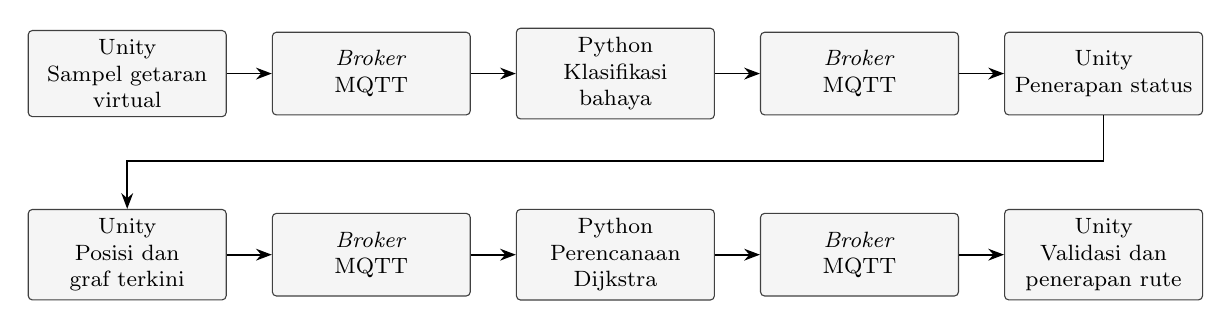
\begin{tikzpicture}[
  flowbox/.style={draw=black!75, rounded corners=1.5pt, fill=black!4,
    minimum width=2.40cm, minimum height=1.05cm, text width=2.28cm,
    align=center, font=\fontsize{8}{9.5}\selectfont},
  flowarrow/.style={-{Stealth[length=2mm]}, semithick}
]
\node[flowbox] (sensor) at (0,2.3) {Unity\\Sampel getaran virtual};
\node[flowbox] (broker-a) at (3.1,2.3) {\emph{Broker}\\MQTT};
\node[flowbox] (classifier) at (6.2,2.3) {Python\\Klasifikasi bahaya};
\node[flowbox] (broker-b) at (9.3,2.3) {\emph{Broker}\\MQTT};
\node[flowbox] (status) at (12.4,2.3) {Unity\\Penerapan status};
\node[flowbox] (request) at (0,0) {Unity\\Posisi dan graf terkini};
\node[flowbox] (broker-c) at (3.1,0) {\emph{Broker}\\MQTT};
\node[flowbox] (planner) at (6.2,0) {Python\\Perencanaan Dijkstra};
\node[flowbox] (broker-d) at (9.3,0) {\emph{Broker}\\MQTT};
\node[flowbox] (apply) at (12.4,0) {Unity\\Validasi dan penerapan rute};
\foreach \a/\b in {sensor/broker-a,broker-a/classifier,classifier/broker-b,broker-b/status,request/broker-c,broker-c/planner,planner/broker-d,broker-d/apply}
  \draw[flowarrow] (\a.east) -- (\b.west);
\draw[flowarrow] (status.south) -- ++(0,-0.58) -| (request.north);
\end{tikzpicture}
\caption{Alur status bahaya dan perencanaan rute pada konfigurasi MQTT. Baris atas menunjukkan klasifikasi input virtual; baris bawah menunjukkan perhitungan dan penerapan rute.}
\label{fig:architecture}
\end{figure}
\subsection*{Pembentukan input bahaya}
Dua belas detektor ditempatkan pada jaringan lorong. Setiap detektor menghasilkan intensitas getaran virtual ternormalisasi pada interval waktu simulasi 0,05 s. Profil normal, waspada, dan bahaya menggunakan intensitas dasar berturut-turut 0,12; 0,58; dan 0,90, dengan variasi deterministik sebesar $\pm$0,04. Sampel ditentukan oleh \emph{seed}, identitas detektor, indeks sampel, dan jadwal profil. Pembentukannya tidak bergantung pada posisi atau kedekatan agen terhadap detektor.

Layanan Python menggunakan ambang 0,45 untuk status waspada dan 0,75 untuk status tertutup, dengan durasi pemenuhan ambang minimum 0,5 s waktu simulasi. Pemulihan dari status waspada menggunakan ambang 0,30 selama 1 s waktu simulasi. Status tertutup dipertahankan hingga sesi direset. Nilai dan ambang tersebut merupakan parameter desain demonstrasi dengan intensitas ternormalisasi, sehingga evaluasi akurasi deteksi longsor menggunakan data sensor terkalibrasi memerlukan penelitian tersendiri.

Skenario acak menggunakan tiga kejadian pada lokasi detektor yang berbeda. Ketika tersedia kandidat yang memenuhi syarat, lokasi kejadian pertama dipilih dari detektor pada rute referensi awal yang, apabila selnya ditutup, masih menyisakan alternatif dari titik awal menuju zona aman. Kejadian berikutnya dipilih dari detektor yang belum digunakan. Dengan demikian, distribusi skenario bersifat kondisional untuk menguji respons terhadap gangguan rute awal. Apabila kandidat pertama tidak tersedia, pemilihan menggunakan kumpulan detektor yang tersedia.

Awal profil waspada pertama berada pada rentang 6--8 s waktu simulasi. Profil bahaya dimulai 4 s setelah awal profil waspada. Profil waspada berikutnya dimulai 6--8 s setelah awal profil bahaya sebelumnya. Pada sumber MQTT, jadwal tersebut menentukan perubahan input getaran; waktu status diterapkan di Unity juga dipengaruhi pemenuhan durasi ambang, pengiriman pesan, dan pemrosesan aplikasi. Jadwal input dan jejak penerapan status dicatat secara terpisah. Dua kontrol fungsional disediakan berupa skenario tanpa bahaya dan skenario berjadwal tetap.

\subsection*{Kebijakan perencanaan rute}
Kebijakan adaptif menggunakan algoritme Dijkstra \cite{haam} untuk mencari lintasan berbiaya minimum dari sel agen saat ini menuju salah satu zona aman. Biaya transisi ke sel tetangga v pada keadaan t dirumuskan sebagai:

\begin{equation}
 c_t(u,v)=6+\lambda\,\mathbf{1}\{v\in W_t\},\qquad v\notin B_t.
 \label{eq:cost}
\end{equation}
dengan $W_t$ sebagai himpunan sel waspada, $B_t$ sebagai himpunan sel tertutup, dan $\lambda$ sebagai penalti waspada. Biaya lintasan merupakan jumlah biaya transisi sepanjang lintasan. Nilai dasar $\lambda$ = 24 setara dengan empat biaya langkah dalam fungsi objektif. Penalti tersebut merupakan bobot heuristik yang memengaruhi keputusan navigasi; interpretasi sebagai probabilitas cedera atau dosis bahaya memerlukan model fisik yang berbeda. Sel waspada masih dapat dipilih apabila alternatif memiliki biaya lebih tinggi, sedangkan sel tertutup dikeluarkan dari pencarian adaptif.

Rute awal kedua kebijakan dihitung oleh layanan Python pada kondisi awal yang sama. Kebijakan statis mempertahankan rute tersebut ketika status bahaya berubah. Kebijakan adaptif mengirimkan permintaan baru setelah pembaruan status dan menerapkan respons yang sesuai dengan posisi serta revisi kondisi terkini. Urutan penelusuran tetangga dan pemecahan biaya sama dibuat deterministik. Kesamaan rute referensi generator dengan rute awal Python diperiksa pada tahap verifikasi.

Selama menunggu respons yang relevan, pergerakan agen dihentikan sementara, sedangkan waktu simulasi dan input bahaya tetap berkembang. Respons yang sudah tidak sesuai dengan posisi atau revisi status ditolak. Permintaan navigasi memiliki batas tunggu 5 s waktu nyata, dengan penyesuaian hitungan \emph{timeout} ketika sesi dijeda. Kegagalan layanan navigasi dicatat sebagai alasan terminasi tersendiri. Kebijakan ini menyebabkan evaluasi mencakup konsekuensi operasional komunikasi dan waktu menunggu, selain keputusan lintasan.

\subsection*{Rancangan eksperimen berpasangan}
Evaluasi utama dilaksanakan menggunakan 30 \emph{seed} yang ditetapkan sebelum rangkaian, yaitu 101--130. Setiap \emph{seed} membentuk satu pasangan sesi adaptif dan statis, sehingga terdapat 60 sesi pada satu topologi; seluruh sesi yang ditetapkan selesai tanpa pengulangan atau pengecualian. Kedua sesi dalam pasangan menggunakan denah, titik awal, zona aman, parameter gerak, penalti, lokasi detektor, dan jadwal input yang sama. Kesetaraan input diperiksa melalui berkas jadwal serta sampel virtual, sementara jejak status digunakan untuk memeriksa perbedaan waktu penerapan akibat komunikasi.

Eksperimen dilaksanakan menggunakan sumber MQTT dengan Python sebagai perencana rute, pengacakan \emph{seed} saat peluncuran dinonaktifkan, dan faktor skala waktu Unity sebesar 1. Program pelaksana eksperimen dijalankan pada salinan proyek dalam mode tanpa tampilan. Ambang perpindahan minimum \texttt{CharacterController} ditetapkan sebesar 0 m agar langkah gerak kecil pada pembaruan berfrekuensi tinggi tetap diterapkan. Target pembaruan ditetapkan sebesar 60 per detik, tetapi frekuensi aktual editor tanpa tampilan dapat melampaui target tersebut. Kondisi perangkat, versi lingkungan perangkat lunak, urutan sesi, dan pengaturan \emph{frame} dicatat sebelum pengambilan data. Pemanasan layanan serta kontrol fungsional dilakukan terpisah dari 60 sesi utama. Urutan adaptif dan statis diseimbangkan antar-\emph{seed} untuk mengurangi keterikatan kebijakan dengan urutan pelaksanaan: \emph{seed} ganjil dimulai dengan adaptif, sedangkan \emph{seed} genap dimulai dengan statis. Batas observasi ditetapkan sebesar 180 s waktu simulasi atau 300 s waktu nyata; sesi yang mencapai batas tersebut dicatat sebagai penghentian administratif. Alur verifikasi, pelaksanaan, dan audit dirangkum pada Gambar~\ref{fig:experiment}.

\begin{figure}[!htbp]
\centering
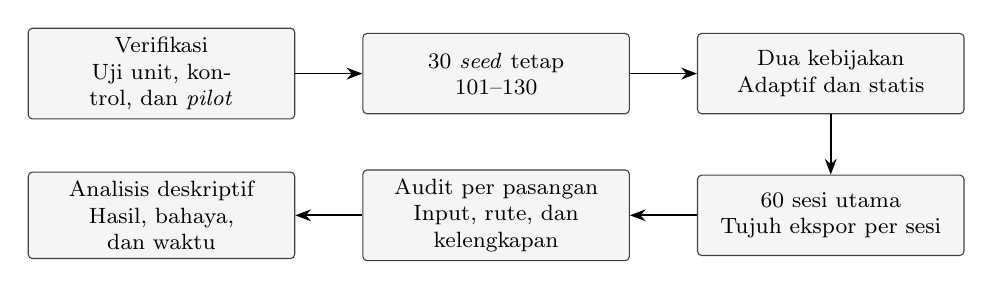
\begin{tikzpicture}[
  stepbox/.style={draw=black!75, rounded corners=1.5pt, fill=black!4,
    minimum width=3.35cm, minimum height=1.02cm, text width=3.15cm,
    align=center, font=\fontsize{8}{9.5}\selectfont},
  flowarrow/.style={-{Stealth[length=2mm]}, semithick}
]
\node[stepbox] (verify) at (0,1.8) {Verifikasi\\Uji unit, kontrol, dan \emph{pilot}};
\node[stepbox] (seeds) at (4.25,1.8) {30 \emph{seed} tetap\\101--130};
\node[stepbox] (policies) at (8.5,1.8) {Dua kebijakan\\Adaptif dan statis};
\node[stepbox] (sessions) at (8.5,0) {60 sesi utama\\Tujuh ekspor per sesi};
\node[stepbox] (audit) at (4.25,0) {Audit per pasangan\\Input, rute, dan kelengkapan};
\node[stepbox] (analysis) at (0,0) {Analisis deskriptif\\Hasil, bahaya, dan waktu};
\draw[flowarrow] (verify.east) -- (seeds.west);
\draw[flowarrow] (seeds.east) -- (policies.west);
\draw[flowarrow] (policies.south) -- (sessions.north);
\draw[flowarrow] (sessions.west) -- (audit.east);
\draw[flowarrow] (audit.west) -- (analysis.east);
\end{tikzpicture}
\caption{Alur eksperimen berpasangan. Kontrol dan \emph{pilot} digunakan untuk verifikasi dan tidak dimasukkan ke dalam 60 sesi utama.}
\label{fig:experiment}
\end{figure}

Seluruh sesi yang direncanakan dipertahankan dalam catatan penelitian, termasuk kegagalan navigasi dan gangguan komunikasi. Alasan terminasi dibedakan antara penutupan pada posisi agen, rute tetap terhalang, tidak ditemukannya lintasan, gangguan navigasi, dan penghentian administratif. Pengulangan akibat gangguan dicatat sebagai percobaan tambahan dan tidak menggantikan catatan awal secara diam-diam. Jumlah 30 pasangan digunakan sebagai rangkaian eksploratif, dengan cakupan interpretasi pada topologi, parameter, dan distribusi skenario yang ditetapkan.

\subsection*{Definisi metrik dan analisis}
Keberhasilan didefinisikan sebagai tercapainya posisi agen pada jarak horizontal kurang dari 1,8 m dari salah satu pusat zona aman. Hasil ini dianalisis bersama indikator kedekatan bahaya, karena tercapainya zona aman tidak mensyaratkan paparan nol. Durasi sesi dihitung dari awal sesi hingga terminasi dan mencakup \emph{briefing} awal 4 s serta waktu menunggu navigasi. Waktu simulasi mengikuti pembaruan \emph{frame} dengan penambahan min(\texttt{Time.deltaTime}, 0,05 s); langkah pengukuran gerak tersebut dibedakan dari interval sampel sensor yang tetap.

Durasi sesi berhasil dilaporkan sebagai waktu hingga mencapai zona aman. Durasi sesi gagal dilaporkan sebagai waktu hingga terminasi dengan alasan kegagalan. Kedua titik akhir pengukuran disajikan terpisah. Agen otomatis yang mengikuti \emph{waypoint} tertutup dihentikan ketika jaraknya terhadap pusat \emph{waypoint} kurang dari 4,2 m. Penutupan pada sel agen menyebabkan penghentian langsung, sementara respons tanpa lintasan menghasilkan alasan tidak ditemukannya rute. Jarak perjalanan dihitung sebagai akumulasi perpindahan horizontal agen. Paparan merupakan akumulasi waktu ketika agen berada pada radius kurang dari 4,5 m dari sedikitnya satu pusat sel tertutup. Kontak menghitung transisi memasuki gabungan zona kedekatan tersebut, dengan tambahan kejadian khusus apabila penutupan terjadi pada sel agen. Keduanya merupakan indikator geometris dalam model.

Jumlah pengalihan rute menghitung perubahan sisa urutan sel atau target zona aman akibat pembaruan bahaya, dengan bagian rute yang sudah dilalui diabaikan. Penerimaan respons yang mempertahankan keputusan rute tidak menambah hitungan pengalihan.

Pengukuran waktu komputasi dibedakan menjadi tiga cakupan. Pertama, durasi pencarian dan rekonstruksi rute Python diukur menggunakan penghitung monotonik pada fungsi perencana rute; \emph{parsing} permintaan, serialisasi respons, dan komunikasi berada di luar pencatat waktu tersebut. Kedua, waktu permintaan hingga penerapan diukur sejak permintaan masuk antrean publikasi Unity sampai respons diterapkan. Ketiga, waktu pembaruan bahaya hingga penerapan rute diukur sejak awal pembaruan bahaya yang belum terselesaikan sampai rute sesuai revisi terkini diterapkan. Perubahan bahaya yang bertumpang tindih dapat tergabung dalam satu interval terakhir ini.

Durasi dihitung menggunakan selisih penghitung lokal pada proses yang sama. Pengukuran sensor fisik sampai tampilan navigasi memerlukan instrumentasi tambahan. Pengukuran rute awal dipisahkan dari perencanaan ulang; waktu perencanaan ulang statis tidak dilaporkan karena kebijakan tersebut tidak menghasilkan respons perencanaan ulang. Sesi dengan jeda atau gangguan komunikasi dianalisis terpisah dari distribusi timing normal.

Analisis deskriptif menyajikan proporsi mencapai zona aman, kategori hasil dalam setiap pasangan, alasan kegagalan, jarak dan waktu menurut hasil, indikator kedekatan bahaya, jumlah pengalihan, serta distribusi waktu komputasi dan penerapan. Pengamatan tiap permintaan tetap dihubungkan dengan sesi asalnya. Perbandingan waktu penyelesaian hanya menggunakan sesi berhasil dan menjelaskan jumlah observasi yang tersedia; apabila suatu kebijakan tidak memiliki sesi berhasil, waktu penyelesaiannya dinyatakan tidak tersedia. Efek pembaruan rute dan penalti waspada belum dapat diisolasi hanya melalui pembandingan adaptif dengan statis.

\subsection*{Verifikasi dan keterlacakan data}
Verifikasi sebelum rangkaian utama dilaksanakan melalui pengujian unit, kontrol tanpa bahaya dan skenario berjadwal pada kedua kebijakan, serta dua pasangan \emph{pilot} acak dengan \emph{seed} 201 dan 202. Pemeriksaan meliputi hasil perencana rute terhadap perhitungan biaya acuan dengan relaksasi independen, validasi respons, perubahan status bahaya, reset sesi, penolakan respons yang sudah tidak relevan, dan batas tunggu ketika \emph{broker} tidak tersedia. Regresi gerak diperiksa terpisah untuk memastikan perpindahan sesuai kecepatan nominal. Tahap ini ditujukan untuk memeriksa kesesuaian perilaku implementasi dengan aturan model; kontrol dan \emph{pilot} tidak dimasukkan ke dalam 60 sesi utama.

Ekspor kontrol dan \emph{pilot} diaudit terhadap identitas sesi, hasil, kelengkapan berkas, kesamaan denah, jadwal, dan rute awal, serta nilai sampel pada indeks waktu simulasi bersama. Kelayakan lintasan dan biaya minimum setiap respons yang diterapkan diperiksa menggunakan \emph{snapshot} permintaannya. Runner rangkaian utama hanya menerima manifest kontrol dan \emph{pilot} beserta hasil audit yang berhasil dengan \emph{fingerprint} sumber identik. Perubahan sumber setelah tahap tersebut mengharuskan verifikasi diulang.

Setiap sesi menyimpan ringkasan hasil, kejadian aktual, denah, jadwal input, konfigurasi, jejak pemrosesan status, dan jejak navigasi. Identitas versi kode dan perangkat pengujian disimpan bersama paket eksperimen. Bukti untuk konfigurasi Python/MQTT berasal dari keluaran rangkaian utama yang menggunakan sumber kode dan konfigurasi identik dengan kontrol serta \emph{pilot} yang lolos. \emph{Snapshot} sumber, \emph{scene} aktual, pengaturan proyek, versi lingkungan, manifest, dan prosedur agregasi disimpan bersama \emph{dataset}.

\FloatBarrier
\section*{Hasil dan Pembahasan}
\subsection*{Verifikasi implementasi dan kelengkapan data}
Pengambilan data utama dilaksanakan setelah pengujian unit, kontrol fungsional, dan \emph{pilot} memenuhi kriteria verifikasi. Dua puluh metode pengujian unit Python berhasil dijalankan, termasuk pemeriksaan biaya minimum pada 81 kombinasi status graf kecil menggunakan implementasi relaksasi terpisah. Kontrol tanpa bahaya menunjukkan bahwa kedua kebijakan dapat mencapai zona aman. Skenario berjadwal dan dua pasangan \emph{pilot} dengan \emph{seed} 201 serta 202 menunjukkan penerapan rute adaptif dan penghentian rute statis sesuai aturan model. Kontrol dan \emph{pilot} tersebut tidak dimasukkan ke dalam hasil 60 sesi utama.

Verifikasi gerak mengidentifikasi bahwa ambang perpindahan minimum \texttt{CharacterController} sebesar 0,001 m mengabaikan sebagian langkah kecil pada pembaruan tanpa tampilan. Setelah ambang ditetapkan sebesar 0 m, regresi terisolasi menghasilkan perpindahan sekitar 2,801 m dalam satu detik gerak, mendekati kecepatan nominal 2,8 m/s. Konfigurasi hasil perbaikan dibekukan sebelum rangkaian utama.

Lingkungan Unity dan komponen informasi navigasi disiapkan untuk didokumentasikan pada Gambar~\ref{fig:unity}. Rangkaian utama menghasilkan 60 sesi lengkap dari 30 pasangan \emph{seed} 101--130. Setiap pasangan menggunakan denah, jadwal input, parameter model, dan rute awal yang sama. Audit ekspor memeriksa kelengkapan tujuh jenis berkas setiap sesi, kelayakan lintasan, dan kesesuaian biaya dengan perhitungan minimum graf. Sebanyak 240 respons diterapkan berhasil diperiksa. Pada waktu observasi bersama, 164.340 sampel virtual dibandingkan dan cocok seluruhnya. Parameter model konsisten pada seluruh konfigurasi sesi, dengan 67 simpul dan 76 sisi tak berarah. Indikator kehilangan data, putus koneksi, kehilangan kemutakhiran setelah siap, dan kegagalan navigasi tidak aktif pada rangkaian utama. Tidak terdapat sesi yang dihentikan oleh batas observasi administratif.

\begin{figure}[!htbp]\centering
\begin{subfigure}[t]{0.24\linewidth}\centering
\includegraphics[width=\linewidth]{fig-unity-a}
\caption{Denah jaringan lorong}\end{subfigure}
\hfill
\begin{subfigure}[t]{0.72\linewidth}\centering
\includegraphics[width=\linewidth]{fig-unity-b}
\caption{Sudut kamera Mode Cerita}\end{subfigure}
\caption{Lingkungan prototipe pada Unity 6000.3.23f1: (a) denah jaringan lorong dengan tiga zona aman (hijau) dan lokasi detektor; (b) sudut kamera Mode Cerita dengan agen pekerja dan jalur evakuasi. Pratinjau editor dari \emph{scene} yang sama dengan rangkaian utama, bukan tangkapan sesi eksperimen.}\label{fig:unity}\end{figure}
\subsection*{Hasil navigasi berpasangan}
Kebijakan adaptif mencapai zona aman pada 30 dari 30 sesi (100,0\%), sedangkan kebijakan statis mencapai zona aman pada 0 dari 30 sesi (0,0\%). Distribusi hasil berpasangan ditampilkan pada Tabel~\ref{tab:paired}. Denominator tetap mencakup seluruh 30 pasangan yang ditetapkan sebelum pengambilan data.

\begin{table}[!htbp]\centering
\caption{Distribusi hasil pada 30 pasangan skenario konfigurasi MQTT.}\label{tab:paired}
\begin{tabularx}{\linewidth}{YYr}\toprule
Hasil adaptif & Hasil statis & Pasangan\\\midrule
Mencapai zona aman & Terhenti karena rute terhalang & 30\\\bottomrule
\end{tabularx}
\vspace{3pt}\par\noindent\raggedright Seluruh pasangan menghasilkan kombinasi hasil tersebut; kombinasi lain tidak teramati.\end{table}

Interpretasi hasil mempertimbangkan pembentukan skenario yang bersifat kondisional. Bahaya pertama dipilih dari detektor pada rute referensi awal yang masih menyisakan alternatif apabila selnya ditutup. Dalam rangkaian ini, lokasi pertama terdiri atas sel (0, 4) pada 15 pasangan; sel (0, 7) pada 15 pasangan. Jejak statis menunjukkan bahwa penutupan lokasi pertama telah diterapkan sebelum penghentian pada seluruh 30 sesi. Dengan demikian, hasil mencerminkan respons kedua kebijakan terhadap gangguan yang sengaja ditempatkan pada rute awal. Proporsi yang diperoleh tidak mengestimasi peluang keberhasilan pada keseluruhan kondisi kecelakaan tambang.

Kebijakan adaptif memperbarui rute ketika status berubah dan menerapkan respons yang sesuai dengan posisi serta revisi terkini. Kebijakan statis mempertahankan rute awal dan dihentikan ketika mendekati \emph{waypoint} yang sudah tertutup. Perbandingan ini menunjukkan manfaat operasional pembaruan rute pada konfigurasi uji. Gambar~\ref{fig:comparison} disediakan untuk dokumentasi respons kedua kebijakan pada \emph{seed} 101. Kontribusi penalti waspada belum dapat dipisahkan dari kontribusi perencanaan ulang karena keduanya hadir bersama pada kebijakan adaptif. Pembandingan tambahan dengan kebijakan reaktif tanpa penalti diperlukan apabila penelitian diarahkan pada isolasi pengaruh masing-masing mekanisme.

\begin{figure}[!htbp]\centering
\begin{subfigure}[t]{0.32\linewidth}\centering
\includegraphics[width=\linewidth]{fig-comparison-a}
\caption{Adaptif, 3,0 s: rute awal}\end{subfigure}
\hfill
\begin{subfigure}[t]{0.32\linewidth}\centering
\includegraphics[width=\linewidth]{fig-comparison-b}
\caption{Adaptif, 10,5 s: D01 tertutup}\end{subfigure}
\hfill
\begin{subfigure}[t]{0.32\linewidth}\centering
\includegraphics[width=\linewidth]{fig-comparison-c}
\caption{Adaptif, 62,7 s: zona aman 3}\end{subfigure}
\par\medskip
\begin{subfigure}[t]{0.32\linewidth}\centering
\includegraphics[width=\linewidth]{fig-comparison-d}
\caption{Statis, 3,0 s: rute awal}\end{subfigure}
\hfill
\begin{subfigure}[t]{0.32\linewidth}\centering
\includegraphics[width=\linewidth]{fig-comparison-e}
\caption{Statis, 10,5 s: D01 tertutup}\end{subfigure}
\hfill
\begin{subfigure}[t]{0.32\linewidth}\centering
\includegraphics[width=\linewidth]{fig-comparison-f}
\caption{Statis, 17,1 s: terhenti}\end{subfigure}
\caption{Respons kebijakan adaptif (a--c) dan statis (d--f) pada skenario terkontrol dengan penutupan pertama D01 di sel (0, 4), sel yang sama dengan lokasi pertama pada 15 pasangan rangkaian utama. Setelah D01 tertutup, kebijakan adaptif memetakan ulang rute hingga mencapai zona aman, sedangkan kebijakan statis mempertahankan rute awal hingga terhenti. Konfigurasi Python/MQTT; waktu pada setiap panel adalah waktu simulasi sesi. Tangkapan berasal dari versi prototipe terbaru yang menambahkan jeda pemeriksaan pada Mode Cerita, sehingga waktunya berbeda dari Tabel~\ref{tab:duration} dan tidak termasuk 60 sesi rangkaian utama.}\label{fig:comparison}\end{figure}
Kebijakan adaptif mencatat 34 pengalihan rute: 26 sesi mengalami satu pengalihan dan 4 sesi mengalami dua pengalihan. Kebijakan statis tidak melakukan pengalihan. Jumlah ini berbeda dari 180 respons perencanaan ulang, karena pembaruan status yang menghasilkan sisa lintasan dan tujuan identik tidak dihitung sebagai perubahan rute.

\subsection*{Durasi, jarak, dan indikator kedekatan bahaya}
Rerata waktu mencapai zona aman pada sesi adaptif berhasil adalah 37,429 s dengan simpangan baku 0,014 s, sedangkan rerata jarak perjalanan adalah 93,449 m. Durasi mencakup \emph{briefing} awal empat detik dan waktu menunggu navigasi. Jarak merupakan akumulasi perpindahan horizontal agen, sehingga tidak disamakan dengan biaya lintasan graf. Ringkasan menurut kebijakan dan hasil disajikan pada Tabel~\ref{tab:duration}.

\begin{table}[!htbp]\centering
\caption{Durasi dan jarak menurut kebijakan serta hasil sesi.}\label{tab:duration}
\setlength{\tabcolsep}{4pt}
\begin{tabularx}{\linewidth}{Yrrrrr}\toprule
Kebijakan dan hasil & $n$ & \shortstack{Rerata\\durasi (s)} & \shortstack{SD\\durasi (s)} & \shortstack{Rerata\\jarak (m)} & \shortstack{Rerata\\kedekatan (s)}\\\midrule
Adaptif, mencapai zona aman & 30 & 37,429 & 0,014 & 93,449 & 0,008\\
Statis, terhenti & 30 & 22,857 & 3,269 & 52,800 & 0,108\\\bottomrule
\end{tabularx}
\vspace{3pt}\par\noindent\raggedright Durasi berhasil berakhir saat zona aman tercapai; durasi terhenti berakhir saat kegagalan. SD: simpangan baku sampel.\end{table}

Tidak terdapat observasi waktu mencapai zona aman pada kebijakan statis. Oleh karena itu, durasi sesi statis yang terhenti tidak digunakan untuk menghitung persentase percepatan evakuasi terhadap kebijakan adaptif.

Keberhasilan mencapai zona aman dianalisis bersama indikator kedekatan bahaya. Indikator ini mengakumulasi waktu ketika agen berada dalam radius kurang dari 4,5 m dari pusat sedikitnya satu sel tertutup. Kontak perimeter menghitung transisi memasuki zona tersebut. Keduanya merupakan ukuran geometris simulasi dan belum menggambarkan dosis paparan ataupun tingkat cedera fisik. Ringkasan seluruh sesi ditampilkan pada Tabel~\ref{tab:proximity}; durasi observasi antar-hasil berbeda karena sesi berhenti ketika titik akhir pengukuran masing-masing tercapai.

\begin{table}[!htbp]\centering
\caption{Kontak perimeter dan akumulasi indikator kedekatan pada rangkaian utama.}\label{tab:proximity}
\begin{tabularx}{\linewidth}{Yrrr}\toprule
Kebijakan & \shortstack{Sesi dengan\\kontak perimeter} & \shortstack{Jumlah\\sesi} & \shortstack{Total indikator\\kedekatan (s)}\\\midrule
Adaptif & 2 & 30 & 0,251\\
Statis & 30 & 30 & 3,228\\\bottomrule
\end{tabularx}\end{table}

Pada \emph{seed} 106, penutupan D02 diterapkan sekitar 33,063 s dan disertai satu kejadian memasuki perimeter kedekatan. Agen tetap mencapai zona aman pada 37,439 s, dengan akumulasi indikator kedekatan 0,197 s. Pada \emph{seed} 122, penutupan D05 diterapkan sekitar 33,266 s dan disertai satu kejadian memasuki perimeter kedekatan. Agen tetap mencapai zona aman pada 37,498 s, dengan akumulasi indikator kedekatan 0,054 s. Pada \emph{seed} 106, permintaan terakhir mencatat posisi pada sel (-4, 6), dengan rute menuju sel (-4, 8) melalui (-4, 7), sementara (-4, 5) sudah tertutup. Contoh ini memperlihatkan bahwa lintasan yang layak pada graf dapat disertai kedekatan geometris terhadap pusat sel tertutup di sekitar lintasan. Pencapaian zona aman dan indikator kedekatan karena itu dipertahankan sebagai dua luaran terpisah. Posisi agen, sel tertutup, serta rute aktif pada contoh tersebut akan ditampilkan dalam dokumentasi Unity pada Gambar~\ref{fig:proximity}.

\begin{figure}[!htbp]\centering
\begin{subfigure}[t]{0.49\linewidth}\centering
\includegraphics[width=\linewidth]{fig-proximity-a}
\caption{30,4 s: D12 tertutup sekitar 4 m dari agen}\end{subfigure}
\hfill
\begin{subfigure}[t]{0.49\linewidth}\centering
\includegraphics[width=\linewidth]{fig-proximity-b}
\caption{57,6 s: zona aman 2, kontak 1}\end{subfigure}
\caption{Ilustrasi pencapaian zona aman yang disertai indikator kedekatan bahaya pada kebijakan adaptif. Penutupan D12 diatur secara manual melalui jadwal pembanding ketika agen berada sekitar 4 m dari sel tersebut; agen tetap mencapai zona aman dengan satu kontak perimeter. Tangkapan dari versi prototipe terbaru untuk dokumentasi, bukan dari rangkaian utama; akumulasi kedekatan pada panel mencakup jeda pemeriksaan sehingga tidak sebanding dengan Tabel~\ref{tab:proximity}.}\label{fig:proximity}\end{figure}
\subsection*{Waktu komputasi dan penerapan rute}
Pengukuran waktu dibedakan antara pencarian serta rekonstruksi rute Python dan durasi sejak permintaan masuk antrean publikasi hingga respons diterapkan di Unity. Distribusi rute awal dan perencanaan ulang disajikan pada Tabel~\ref{tab:timing}. Setiap pengamatan dihubungkan dengan sesi asalnya. Persentil ke-95 dihitung melalui interpolasi linear pada observasi yang diurutkan. Pengamatan permintaan berulang di dalam sesi tidak diperlakukan sebagai replikasi eksperimen yang independen.

\begin{table}[!htbp]\centering
\caption{Waktu pencarian Python dan antrean sampai penerapan respons di Unity.}\label{tab:timing}
\setlength{\tabcolsep}{3pt}
\begin{tabularx}{\linewidth}{Yrrrrrr}\toprule
Kebijakan / fase & $n$ & \multicolumn{2}{c}{Pencarian (ms)} & \multicolumn{3}{c}{Antrean--penerapan (ms)}\\
\cmidrule(lr){3-4}\cmidrule(lr){5-7}
 & & Median & P95 & Median & P95 & Maksimum\\\midrule
Adaptif / rute awal & 30 & 0,0434 & 0,0649 & 11,8501 & 13,1078 & 13,1979\\
Adaptif / perencanaan ulang & 180 & 0,0365 & 0,0633 & 9,9415 & 12,3817 & 25,9661\\
Statis / rute awal & 30 & 0,0482 & 0,0602 & 11,8871 & 13,2151 & 13,3019\\\bottomrule
\end{tabularx}
\vspace{3pt}\par\noindent\raggedright $n$: respons yang diterapkan; P95: persentil ke-95. Kebijakan statis tidak memiliki pengamatan perencanaan ulang.\end{table}

Tidak terdapat pengamatan perencanaan ulang pada kebijakan statis; waktu komputasi rute awalnya tetap ditampilkan secara terpisah. Ringkasan timing hanya mencakup respons yang diterapkan; permintaan terantre, respons ditolak, dan permintaan yang digantikan tetap tersimpan dalam jejak terpisah.

Maksimum waktu dari penerapan pembaruan status bahaya di Unity hingga penerapan rute yang relevan pada seluruh sesi adaptif adalah 26,1028 ms. Titik akhir ini berada setelah klasifikasi dan pengiriman status, sehingga tidak mencakup keseluruhan rentang sejak stimulus sensor virtual. Selisih \emph{timestamp} dihitung pada jam lokal yang sama untuk setiap cakupan. Waktu respons pada \emph{broker} \emph{loopback} dan Unity tanpa tampilan belum mengukur latensi jaringan tambang, perangkat UWB, atau tampilan navigasi fisik.

\subsection*{Cakupan interpretasi dan pengembangan lanjutan}
Hasil mendukung kesesuaian implementasi pertukaran status dan rute antara Unity serta proses Python pada konfigurasi yang diuji. Pembedaan antara pemeriksaan implementasi dan ketepatan model untuk domain penggunaan mengikuti pembahasan verifikasi serta validasi simulasi oleh Sargent \cite{fonseca}. Representasi bahaya dalam penelitian ini berupa profil getaran ternormalisasi dan penutupan sel sintetis. Posisi agen diperoleh dari koordinat internal Unity. Keterwakilan bahaya tambang nyata dan ketelitian lokalisasi UWB memerlukan evaluasi tersendiri.

Eksperimen menggunakan satu topologi dan satu agen otomatis dengan kecepatan nominal tetap. Tiga puluh pasangan diperlakukan sebagai rangkaian eksploratif pada daftar \emph{seed} yang ditetapkan, dengan analisis deskriptif. Generalisasi ke topologi lain, variasi parameter, hambatan kapasitas lorong, atau perilaku multiagen belum ditentukan oleh hasil ini. Pengujian juga belum mencakup penerapan pada kontainer, pemrosesan pada perangkat \emph{edge} fisik, maupun putus koneksi yang disengaja di tengah sesi pengukuran normal.

Paket replikasi menyimpan sumber kode, \emph{scene} aktual, pengaturan proyek, konfigurasi lingkungan, daftar \emph{seed}, manifest, ekspor sesi, dan prosedur agregasi. Pelaporan kondisi eksperimen serta perangkat lunak tersebut mendukung prinsip keterlacakan dan replikasi yang ditekankan dalam pedoman STRESS \cite{huang}. Studi berikutnya dapat memisahkan efek perencanaan ulang dan penalti waspada melalui \emph{baseline} reaktif, memperluas topologi serta rentang parameter, kemudian memasukkan galat lokalisasi dan karakteristik komunikasi perangkat fisik sesuai tujuan penggunaannya.

\FloatBarrier
\section*{Kesimpulan}
Penelitian ini menghasilkan prototipe simulasi navigasi adaptif yang menghubungkan Unity, \emph{broker} MQTT, serta proses Python untuk klasifikasi status bahaya dan perencanaan rute. Verifikasi menunjukkan kesesuaian respons dengan aturan graf dan biaya, kelengkapan ekspor, serta kesetaraan input pada pasangan eksperimen. Pada 30 pasangan skenario gangguan rute awal dalam satu topologi, kebijakan adaptif mencapai zona aman pada 30 sesi, sedangkan kebijakan statis mencapai zona aman pada 0 sesi. Rerata waktu mencapai zona aman pada sesi adaptif berhasil adalah 37,429 s.

Temuan menunjukkan kemampuan pembaruan rute pada konfigurasi uji yang ditetapkan. Pencapaian zona aman tetap dibedakan dari indikator kedekatan bahaya; 2 sesi adaptif mencatat kontak perimeter sekaligus mencapai zona aman. Cakupan hasil terbatas pada bahaya sintetis, posisi virtual yang diketahui, satu agen, serta komunikasi antarpemroses pada komputer yang sama. Variasi topologi, \emph{baseline} reaktif, perilaku multiagen, ketidakpastian posisi, dan pengujian komunikasi serta sensor fisik merupakan arah pengembangan untuk menilai kesesuaian sistem pada domain penggunaan yang lebih luas.

\FloatBarrier
\begin{thebibliography}{11}
\setlength{\itemsep}{2pt}\setlength{\parskip}{0pt}
\bibitem{jha} A. Jha, A. Verburg, and P. Tukkaraja, ``Internet of Things-Based Command Center to Improve Emergency Response in Underground Mines,'' \emph{Safety and Health at Work}, vol. 13, no. 1, pp. 40--50, 2022, doi: \href{https://doi.org/10.1016/j.shaw.2021.10.003}{10.1016/j.shaw.2021.10.003}.
\bibitem{meij} R. Meij, M. Soleymani Shishvan, and J. Sattarvand, ``The Development of a New Smart Evacuation Modeling Technique for Underground Mines Using Mathematical Programming,'' \emph{Mining}, vol. 4, no. 1, pp. 106--119, 2024, doi: \href{https://doi.org/10.3390/mining4010008}{10.3390/mining4010008}.
\bibitem{bi} L. Bi, Y. Liu, D. Zhong, and L. Wen, ``Multi-Objective Real-Time Planning of Evacuation Routes for Underground Mine Fires,'' \emph{Applied Sciences}, vol. 14, no. 17, Art. no. 7521, 2024, doi: \href{https://doi.org/10.3390/app14177521}{10.3390/app14177521}.
\bibitem{augustine} P. C. Augustine, A. Moniri-Morad, M. Shahsavar, and J. Sattarvand, ``Investigating the Effect of Human Factors on the Underground Mine Evacuation Process Using Agent-Based Simulation,'' \emph{Applied Sciences}, vol. 14, no. 24, Art. no. 11773, 2024, doi: \href{https://doi.org/10.3390/app142411773}{10.3390/app142411773}.
\bibitem{ziegler} M. Ziegler, A. E. Kianfar, T. Hartmann, and E. Clausen, ``Development and Evaluation of a UWB-Based Indoor Positioning System for Underground Mine Environments,'' \emph{Mining, Metallurgy \& Exploration}, vol. 40, no. 4, pp. 1021--1040, 2023, doi: \href{https://doi.org/10.1007/s42461-023-00797-z}{10.1007/s42461-023-00797-z}.
\bibitem{paakkonen} P. Pääkkönen, S. Horsmanheimo, D. Pakkala, L. Tuomimäki, and J. Backman, ``Reference Architecture Design and Evaluation for Digitalization of Underground Mining,'' \emph{Internet of Things}, vol. 26, Art. no. 101238, 2024, doi: \href{https://doi.org/10.1016/j.iot.2024.101238}{10.1016/j.iot.2024.101238}.
\bibitem{he} P. He, Y. Wang, G. Zheng, and H. Zhou, ``Design and Implementation of an Edge Computing-Based Underground IoT Monitoring System,'' \emph{Mining}, vol. 5, no. 3, Art. no. 54, 2025, doi: \href{https://doi.org/10.3390/mining5030054}{10.3390/mining5030054}.
\bibitem{saha} N. Saha, P. Paul, K. Ji, and R. Harik, ``Performance evaluation framework of MQTT client libraries for IoT applications in manufacturing,'' \emph{Manufacturing Letters}, vol. 41, pp. 1237--1245, 2024, doi: \href{https://doi.org/10.1016/j.mfglet.2024.09.150}{10.1016/j.mfglet.2024.09.150}.
\bibitem{haam} S. Haam, H. Kim, M. Yoo, and W. S. Song, ``Optimal additional evacuation route analysis in deep underground station structures using Dijkstra's algorithm,'' \emph{Developments in the Built Environment}, vol. 24, Art. no. 100784, 2025, doi: \href{https://doi.org/10.1016/j.dibe.2025.100784}{10.1016/j.dibe.2025.100784}.
\bibitem{fonseca} P. Fonseca i Casas, ``A Continuous Process for Validation, Verification, and Accreditation of Simulation Models,'' \emph{Mathematics}, vol. 11, no. 4, Art. no. 845, 2023, doi: \href{https://doi.org/10.3390/math11040845}{10.3390/math11040845}.
\bibitem{huang} Y. Huang and D. Cetinkaya, ``Advancing reproducibility and replicability in simulation: Challenges and opportunities,'' \emph{SIMULATION}, vol. 102, no. 9, 2026, doi: \href{https://doi.org/10.1177/00375497261444678}{10.1177/00375497261444678}.
\end{thebibliography}

\clearpage
\section*{Lampiran}
\subsection*{Ringkasan data 30 pasangan eksperimen}
Tabel~\ref{tab:appendix} memuat seluruh \emph{seed} yang ditetapkan sebelum pengambilan data. Setiap baris mewakili satu pasangan sesi dengan input identik pada indeks pengamatan bersama. Nilai 0,000 pada waktu kedekatan menyatakan tidak adanya waktu yang terukur di dalam radius indikator pada sesi tersebut; nilai ini bukan data hilang. Seluruh sesi adaptif mencapai zona aman dan seluruh sesi statis terhenti dengan alasan rute tetap terhalang. $t_A$ merupakan durasi sampai zona aman pada kebijakan adaptif; $t_S$ merupakan durasi sampai penghentian pada kebijakan statis. $d_A$ dan $d_S$ menyatakan jarak horizontal. $e_A$ dan $e_S$ menyatakan akumulasi waktu kedekatan geometris. $r_A$ menunjukkan pengalihan rute adaptif. Seluruh sesi statis memiliki satu kontak perimeter dan nol pengalihan; kontak adaptif hanya tercatat pada \emph{seed} 106 dan 122. Nilai ditampilkan dengan pembulatan tiga desimal; agregasi menggunakan angka asli.

\setlength{\tabcolsep}{4pt}
\begin{longtable}{rrrrrrrr}
\caption{Data per pasangan pada konfigurasi Python/MQTT.}\label{tab:appendix}\\
\toprule
Seed & $t_A$ (s) & $t_S$ (s) & $d_A$ (m) & $d_S$ (m) & $e_A$ (s) & $e_S$ (s) & $r_A$\\\midrule
\endfirsthead
\multicolumn{8}{c}{Tabel \thetable. Lanjutan}\\\toprule
Seed & $t_A$ (s) & $t_S$ (s) & $d_A$ (m) & $d_S$ (m) & $e_A$ (s) & $e_S$ (s) & $r_A$\\\midrule
\endhead
\bottomrule\endfoot
101 & 37,418 & 19,643 & 93,437 & 43,800 & 0,000 & 0,108 & 1\\
102 & 37,422 & 19,643 & 93,435 & 43,800 & 0,000 & 0,107 & 2\\
103 & 37,428 & 26,071 & 93,448 & 61,800 & 0,000 & 0,107 & 1\\
104 & 37,420 & 19,643 & 93,436 & 43,801 & 0,000 & 0,108 & 1\\
105 & 37,424 & 26,072 & 93,448 & 61,800 & 0,000 & 0,108 & 1\\
106 & 37,439 & 19,643 & 93,434 & 43,800 & 0,197 & 0,107 & 1\\
107 & 37,430 & 26,072 & 93,447 & 61,801 & 0,000 & 0,108 & 1\\
108 & 37,429 & 19,643 & 93,436 & 43,800 & 0,000 & 0,108 & 1\\
109 & 37,421 & 26,072 & 93,448 & 61,800 & 0,000 & 0,108 & 1\\
110 & 37,431 & 19,643 & 93,435 & 43,800 & 0,000 & 0,108 & 1\\
111 & 37,426 & 26,072 & 93,447 & 61,800 & 0,000 & 0,108 & 1\\
112 & 37,420 & 19,643 & 93,436 & 43,800 & 0,000 & 0,108 & 2\\
113 & 37,420 & 26,071 & 93,447 & 61,799 & 0,000 & 0,108 & 1\\
114 & 37,421 & 19,643 & 93,436 & 43,801 & 0,000 & 0,108 & 1\\
115 & 37,425 & 26,072 & 93,447 & 61,800 & 0,000 & 0,108 & 1\\
116 & 37,430 & 19,643 & 93,437 & 43,800 & 0,000 & 0,108 & 1\\
117 & 37,429 & 26,072 & 93,449 & 61,801 & 0,000 & 0,108 & 1\\
118 & 37,414 & 19,643 & 93,437 & 43,801 & 0,000 & 0,108 & 1\\
119 & 37,423 & 26,072 & 93,447 & 61,800 & 0,000 & 0,107 & 1\\
120 & 37,426 & 19,643 & 93,438 & 43,800 & 0,000 & 0,108 & 1\\
121 & 37,424 & 26,072 & 93,447 & 61,801 & 0,000 & 0,108 & 1\\
122 & 37,498 & 19,643 & 93,653 & 43,800 & 0,054 & 0,108 & 2\\
123 & 37,442 & 26,072 & 93,449 & 61,801 & 0,000 & 0,108 & 1\\
124 & 37,427 & 26,072 & 93,447 & 61,800 & 0,000 & 0,108 & 1\\
125 & 37,435 & 19,643 & 93,437 & 43,800 & 0,000 & 0,108 & 1\\
126 & 37,426 & 26,072 & 93,448 & 61,800 & 0,000 & 0,108 & 1\\
127 & 37,433 & 19,643 & 93,436 & 43,801 & 0,000 & 0,108 & 1\\
128 & 37,430 & 26,072 & 93,447 & 61,800 & 0,000 & 0,108 & 1\\
129 & 37,428 & 19,643 & 93,437 & 43,800 & 0,000 & 0,108 & 1\\
130 & 37,428 & 26,072 & 93,446 & 61,800 & 0,000 & 0,107 & 2\\
\end{longtable}

% CATATAN PENYUNTING: semua placeholder perlu diganti gambar aktual sebelum pengumpulan.
% Margin mengikuti instruksi tertulis template, bukan properti DOCX yang berbeda.
\end{document}
